\documentclass[12pt,letterpaper]{article}
\usepackage{graphicx,textcomp}
\usepackage{natbib}
\usepackage{setspace}
\usepackage{fullpage}
\usepackage{color}
\usepackage[reqno]{amsmath}
\usepackage{amsthm}
\usepackage{fancyvrb}
\usepackage{amssymb,enumerate}
\usepackage[all]{xy}
\usepackage{endnotes}
\usepackage{lscape}
\newtheorem{com}{Comment}
\usepackage{float}
\usepackage{hyperref}
\newtheorem{lem} {Lemma}
\newtheorem{prop}{Proposition}
\newtheorem{thm}{Theorem}
\newtheorem{defn}{Definition}
\newtheorem{cor}{Corollary}
\newtheorem{obs}{Observation}
\usepackage[compact]{titlesec}
\usepackage{dcolumn}
\usepackage{tikz}
\usetikzlibrary{arrows}
\usepackage{multirow}
\usepackage{xcolor}
\newcolumntype{.}{D{.}{.}{-1}}
\newcolumntype{d}[1]{D{.}{.}{#1}}
\definecolor{light-gray}{gray}{0.65}
\usepackage{url}
\usepackage{listings}
\usepackage{color}

\definecolor{codegreen}{rgb}{0,0.6,0}
\definecolor{codegray}{rgb}{0.5,0.5,0.5}
\definecolor{codepurple}{rgb}{0.58,0,0.82}
\definecolor{backcolour}{rgb}{0.95,0.95,0.92}

\lstdefinestyle{mystyle}{
	backgroundcolor=\color{backcolour},   
	commentstyle=\color{codegreen},
	keywordstyle=\color{magenta},
	numberstyle=\tiny\color{codegray},
	stringstyle=\color{codepurple},
	basicstyle=\footnotesize,
	breakatwhitespace=false,         
	breaklines=true,                 
	captionpos=b,                    
	keepspaces=true,                 
	numbers=left,                    
	numbersep=5pt,                  
	showspaces=false,                
	showstringspaces=false,
	showtabs=false,                  
	tabsize=2
}
\lstset{style=mystyle}
\newcommand{\Sref}[1]{Section~\ref{#1}}
\newtheorem{hyp}{Hypothesis}

\title{Problem Set 4}
\date{Submitted: April 6, 2023}
\author{Jack Merriman}


\begin{document}
	\maketitle
\section*{Question 1} 

\lstinputlisting[language = R, firstline=10, lastline=14]{PS4.R}

% Table created by stargazer v.5.2.3 by Marek Hlavac, Social Policy Institute. E-mail: marek.hlavac at gmail.com
% Date and time: Thu, Apr 06, 2023 - 13:49:06
\begin{table}[!htbp] \centering   \caption{}   \label{} \begin{tabular}{@{\extracolsep{5pt}}lc} \\[-1.8ex]\hline \hline \\[-1.8ex]  & \multicolumn{1}{c}{\textit{Dependent variable:}} \\ \cline{2-2} \\[-1.8ex] & survival \\ \hline \\[-1.8ex]  m.age & 0.008$^{***}$ \\   & (0.002) \\   & \\  sexfemale & $-$0.082$^{***}$ \\   & (0.027) \\   & \\ \hline \\[-1.8ex] Observations & 26,574 \\ R$^{2}$ & 0.001 \\ Max. Possible R$^{2}$ & 0.986 \\ Log Likelihood & $-$56,503.480 \\ Wald Test & 22.520$^{***}$ (df = 2) \\ LR Test & 22.518$^{***}$ (df = 2) \\ Score (Logrank) Test & 22.530$^{***}$ (df = 2) \\ \hline \hline \\[-1.8ex] \textit{Note:}  & \multicolumn{1}{r}{$^{*}$p$<$0.1; $^{**}$p$<$0.05; $^{***}$p$<$0.01} \\ \end{tabular} \end{table} 

\noindent Our coefficients are statistically significant at $p<0.01$ as shown by the triple asterisks in the stargazer plot, we will use \texttt{anova} against a null model to conduct a $\chi^2$ test on the model:

\lstinputlisting[language = R, firstline=16, lastline=18]{PS4.R}

% Table created by stargazer v.5.2.3 by Marek Hlavac, Social Policy Institute. E-mail: marek.hlavac at gmail.com% Date and time: Thu, Apr 06, 2023 - 14:29:11
\begin{table}[!htbp] \centering   \caption{}   \label{} \begin{tabular}{@{\extracolsep{5pt}}lccccc} \\[-1.8ex]\hline \hline \\[-1.8ex] Statistic & \multicolumn{1}{c}{N} & \multicolumn{1}{c}{Mean} & \multicolumn{1}{c}{St. Dev.} & \multicolumn{1}{c}{Min} & \multicolumn{1}{c}{Max} \\ \hline \\[-1.8ex] loglik & 2 & $-$56,509.110 & 7.961 & $-$56,514.740 & $-$56,503.480 \\ Chisq & 1 & 22.518 &  & 22.518 & 22.518 \\ Df & 1 & 2.000 &  & 2 & 2 \\ Pr(\textgreater \textbar Chi\textbar ) & 1 & 0.00001 &  & 0.00001 & 0.00001 \\ \hline \\[-1.8ex] \end{tabular} \end{table} 

\noindent We can see the p-value is infinitesimally small, and therefore our model is a good predictor of survival.\\

\noindent With our model and its coefficients statistically significant, we can interpret the coefficients with as such:\\

\indent \texttt{m.age}: Holding sex constant, an increase of one year in the age of the child's mother is associated with a $0.008$ increase in the expected log of the hazard rate for the child.\\

\indent \texttt{sexfemale}: Holding the age of the child's mother constant, girls have an average decrease of $0.082$ in their expected log of the hazard rate relative to boys.\\

\noindent We can further our interpretations by exponentiating the coefficients to examine the hazard ratios themselves:

\lstinputlisting[language = R, firstline=20, lastline=21]{PS4.R}

% Table created by stargazer v.5.2.3 by Marek Hlavac, Social Policy Institute. E-mail: marek.hlavac at gmail.com
% Date and time: Thu, Apr 06, 2023 - 14:42:20
\begin{table}[!htbp] \centering   \caption{}   \label{} \begin{tabular}{@{\extracolsep{5pt}} cc} \\[-1.8ex]\hline \hline \\[-1.8ex] m.age & sexfemale \\ \hline \\[-1.8ex] $1.008$ & $0.921$ \\ \hline \\[-1.8ex] \end{tabular} \end{table} 

\indent \texttt{m.age}: Holding sex constant, an increase of one year in the age of the child's mother is associated with a $0.8\%$ increase in the likelihood of the child dying.\\

\indent \texttt{sexfemale}: Holding the age of the child's mother constant, girls are 8\% less likely to die than boys.\\

\noindent Although there is no theoretical reason to believe that an interaction effect would increase the predictive power of the model, we will create a second interactive model to test:

\lstinputlisting[language = R, firstline=23, lastline=25]{PS4.R}

% Table created by stargazer v.5.2.3 by Marek Hlavac, Social Policy Institute. E-mail: marek.hlavac at gmail.com
% Date and time: Thu, Apr 06, 2023 - 14:56:58
\begin{table}[!htbp] \centering   \caption{}   \label{} \begin{tabular}{@{\extracolsep{5pt}}lc} \\[-1.8ex]\hline \hline \\[-1.8ex]  & \multicolumn{1}{c}{\textit{Dependent variable:}} \\ \cline{2-2} \\[-1.8ex] & survival \\ \hline \\[-1.8ex]  m.age & 0.007$^{**}$ \\   & (0.003) \\   & \\  sexfemale & $-$0.127 \\   & (0.140) \\   & \\  m.age:sexfemale & 0.001 \\   & (0.004) \\   & \\ \hline \\[-1.8ex] Observations & 26,574 \\ R$^{2}$ & 0.001 \\ Max. Possible R$^{2}$ & 0.986 \\ Log Likelihood & $-$56,503.430 \\ Wald Test & 22.530$^{***}$ (df = 3) \\ LR Test & 22.624$^{***}$ (df = 3) \\ Score (Logrank) Test & 22.562$^{***}$ (df = 3) \\ \hline \hline \\[-1.8ex] \textit{Note:}  & \multicolumn{1}{r}{$^{*}$p$<$0.1; $^{**}$p$<$0.05; $^{***}$p$<$0.01} \\ \end{tabular} \end{table} 

\noindent We observe that the interaction term in the model (\texttt{m.age:sexfemale}) is not statistically significant, and that the sex term has lost its statistical significance. We will conduct another $\chi^2$ test to see if the model as a whole is more predictive, to be sure.

\lstinputlisting[language = R, firstline=26, lastline=27]{PS4.R}
\newpage
% Table created by stargazer v.5.2.3 by Marek Hlavac, Social Policy Institute. E-mail: marek.hlavac at gmail.com
% Date and time: Thu, Apr 06, 2023 - 15:02:53
\begin{table}[!htbp] \centering   \caption{}   \label{} \begin{tabular}{@{\extracolsep{5pt}}lccccc} \\[-1.8ex]\hline \hline \\[-1.8ex] Statistic & \multicolumn{1}{c}{N} & \multicolumn{1}{c}{Mean} & \multicolumn{1}{c}{St. Dev.} & \multicolumn{1}{c}{Min} & \multicolumn{1}{c}{Max} \\ \hline \\[-1.8ex] loglik & 2 & $-$56,503.460 & 0.038 & $-$56,503.480 & $-$56,503.430 \\ Chisq & 1 & 0.106 &  & 0.106 & 0.106 \\ Df & 1 & 1.000 &  & 1 & 1 \\ Pr(\textgreater \textbar Chi\textbar ) & 1 & 0.744 &  & 0.744 & 0.744 \\ \hline \\[-1.8ex] \end{tabular} \end{table} 

\noindent With a p-value of $0.74$, the model does not pass any significant critical threshold, so we can reject it being more predictive than the existing model which also has significant coefficients.

\newpage
\noindent We are satisfied with the additive predictive power of the mother's age and the child's sex on their hazard ratio. Below are plots illustrating predicted values of the model:

\lstinputlisting[language = R, firstline=29, lastline=34]{PS4.R}
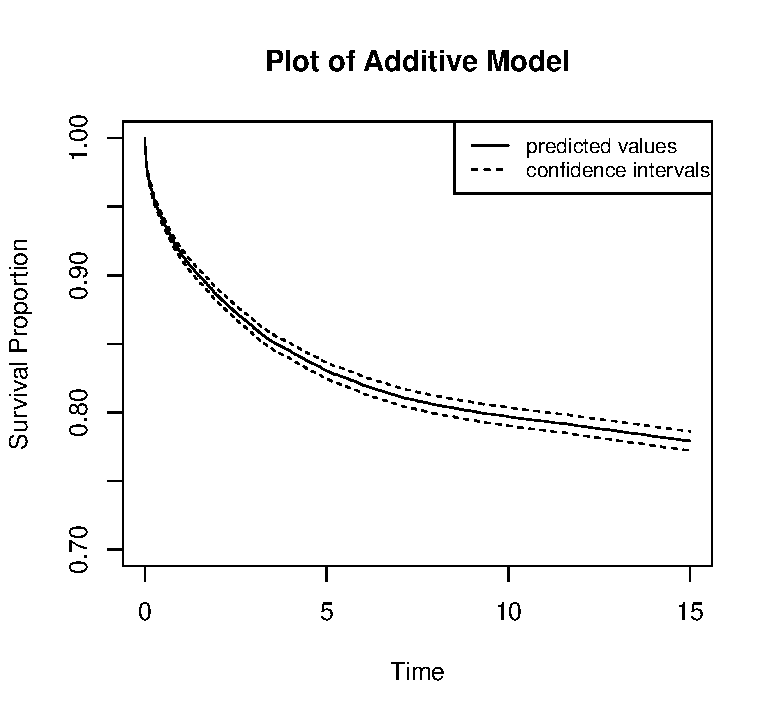
\includegraphics{plot1.pdf}

\newpage
\lstinputlisting[language = R, firstline=36, lastline=37]{PS4.R}
\begin{BVerbatim}
16   17   18   19   20   21   22   23   24   25   26   27   28   29   30
 5   12   66  142  260  438  606  846  999 1143 1250 1302 1400 1444 1490

  31   32   33   34   35   36   37   38  39   40   41   42   43   44   45 
1434 1435 1374 1439 1259 1285 1139 1122 997  859  818  638  507  377  247

 46   47   48   49   51
132   66   32    9    2 
\end{BVerbatim}
\lstinputlisting[language = R, firstline=38, lastline=44]{PS4.R}
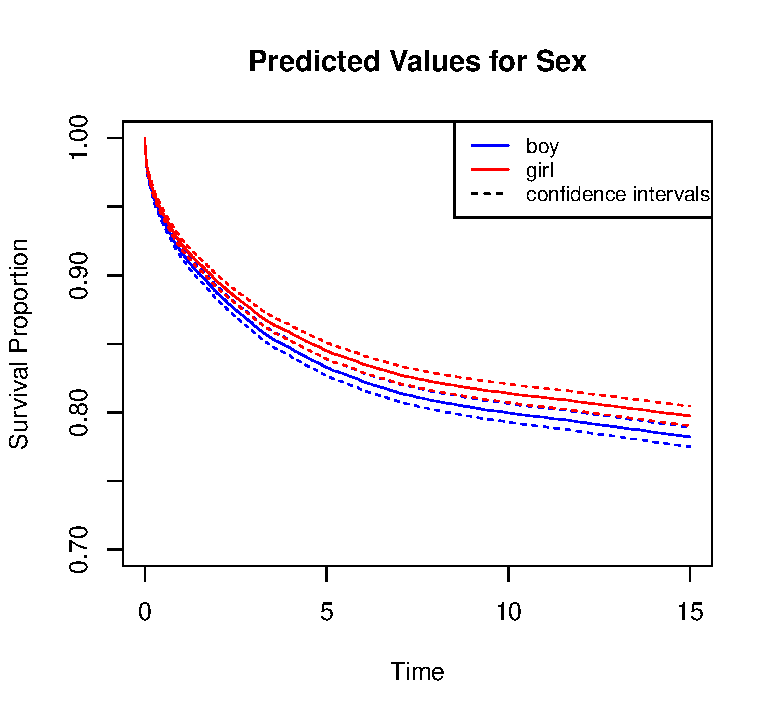
\includegraphics{plot2.pdf}

\newpage
\lstinputlisting[language = R, firstline=46, lastline=54]{PS4.R}
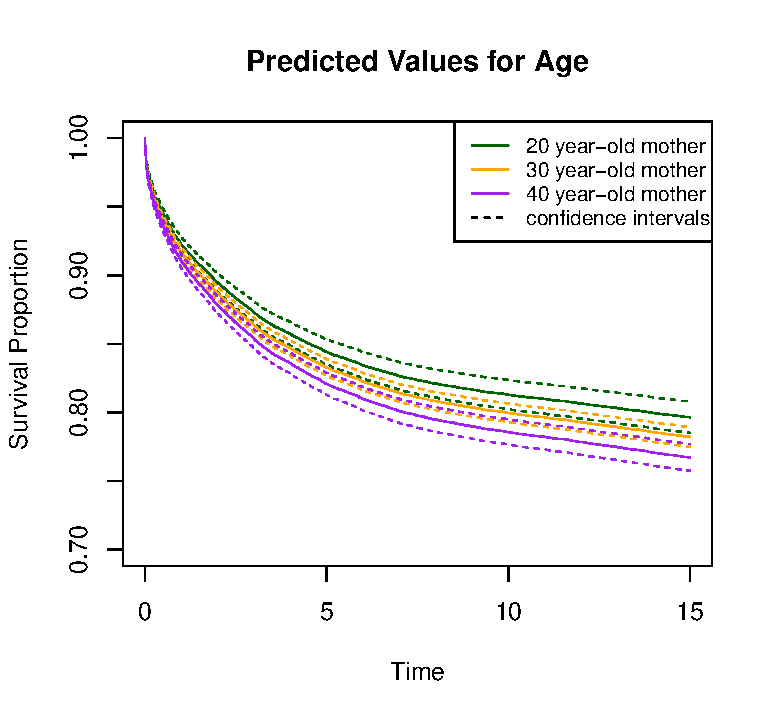
\includegraphics{plot3.pdf}
\end{document}
